\documentclass[12pt]{article}

% title
\title{PHYS 437 HW 1}
\author{Michael Cardiff}
\date{\today}

% science symbols 
\usepackage{amsmath}
\usepackage{amssymb}
\usepackage{physics}

% general pretty stuff
\usepackage{bm}
\usepackage{float}
\usepackage{enumitem}
\usepackage{graphicx}

% figures
\graphicspath{ {./figs/} }
\newcommand{\fig}[3]{
  \begin{figure}[H]
    \centering\includegraphics[width=#1cm]{#2}\caption{#3}
  \end{figure}}

\newcommand{\uv}[1]{\hat{\vb{#1}}}

\renewcommand{\L}{\mathcal{L}}

\begin{document}
\maketitle
\section*{Question 1}
Without loss of generality we can assume that the side length of the cube is 1. From there we see that we need to find the angle between the two red lines in the following figures:
\fig{8.0}{tetrahedral.png}{The Depiction of Tetrahedral Bond Angles by the Body Diagonals of a Cube}
We can make this a bit simpler in terms of the vectors by seeing the symmetry of the situation, and seeing that if we find the angle between the vertical axis (labelled $z$ by Kittel) and one of the red lines, we have half of the required angle. Hence we have the following triangle:
\fig{5.0}{triangle1.png}{Cross section of the above figure}
In the above figure, the red line is the same as in the first one, the blue line is one of the face diagonals, and the thin black one is a side length, and the arc is $\frac{\theta}{2}$. By constructing the unit vector represented by the red line we can find the angle using the following relationship:
\begin{equation*}
  \vb{\hat{a}}\vdot\vb{\hat{b}}=\cos\phi
\end{equation*}
In this case $\phi=\frac{\theta}{2}$. The vector for the corner of the cube is clearly just the addition of the three basic unit vectors, we shall call it $\vb{d}$:
\begin{equation*}
  \vb{d}=\vb{\hat{x}+\hat{y}+\hat{z}}
\end{equation*}
And the other vector, $\vb{a}$ is simply:
\begin{equation*}
  \vb{a}=\vb{\hat{z}}
\end{equation*}
This is already a unit vector, the other one is not normalized, we can normalize it fairly easily, by remembering that the length of the body diagonal should be $\sqrt{3}$ so the unit vector $\vb{\hat{d}}$ is:
\begin{equation*}
  \vb{\hat{d}}=\frac{1}{\sqrt{3}}\qty(\vb{\hat{x}+\hat{y}+\hat{z}})
\end{equation*}
Hence the cosine of $\frac{\theta}{2}$ is:
\begin{equation*}
  \cos\frac{\theta}{2}=\vb{a}\vdot\vb{\hat{d}}=\frac{1}{\sqrt{3}}
\end{equation*}
Solving for $\theta$:
\begin{equation*}
  \theta=2\arccos\frac{1}{\sqrt{3}}
\end{equation*}
Numerically evaluating using a calculator gives:
\begin{equation*}
  \boxed{\theta\approx109.471^\circ}
\end{equation*}
\section*{Question 2}
This is a simple question of changing from the standard cubic basis $\{a_i\}$:
\begin{align*}
  \vb{a}_1=a\vu{x}\quad\vb{a}_2=a\vu{y}\quad\vb{a}_3=a\vu{z}
\end{align*}
To the new basis $\{b_i\}$:
\begin{align*}
  \vb{b}_1=\frac{a}{2}\qty(\vu{x}+\vu{y})\quad
  \vb{b}_2=\frac{a}{2}\qty(\vu{y}+\vu{z})\quad
  \vb{b}_3=\frac{a}{2}\qty(\vu{z}+\vu{x})
\end{align*}
The objective is to write the vectors $\vb{a}_1$ and $\vb{a}_3$ in terms of these new vectors $\{b_i\}$. Essentially we need to find a linear combination of these vectors such that we are left only with either an $a\vu{x}$ or $a\vu{z}$. We can do this by adding two of the $b$ vectors and subtracting, for example we can get $\vb{a}_1$ in the following way:
\begin{align*}
  \vb{b}_1-\vb{b}_2+\vb{b}_3&=
  \frac{a}{2}\qty(\vu{x}+\vu{y}-\vu{y}-\vu{z}+\vu{z}+\vu{x})\\
  &=\frac{a}{2}\qty(2\vu{x})=a\vu{x}=\vb{a}_1
\end{align*}
Thus the indices for the new basis would be $(1,-1,1)$ for the original basis $(1,0,0)$ plane.

We can do a similar process for the $(0,0,1)$ plane, but instead subtracting $\vb{b}_1$ and adding the other two:
\begin{align*}
  -\vb{b}_1+\vb{b}_2+\vb{b}_3&=
  \frac{a}{2}\qty(-\vu{x}-\vu{y}+\vu{y}+\vu{z}+\vu{z}+\vu{x})\\
  &=\frac{a}{2}\qty(2\vu{z})=a\vu{x}=\vb{a}_3
\end{align*}
Hence the $(0,0,1)$ plane now has the indices $(-1,1,1)$
\section*{Question 3}
Ideal hexagonal close packing looks like the following:

\fig{8.0}{hcp1.png}{Hexagonal Close Packing}

We notice that a set of 3 of the red dots and 1 of the green dots will form a tetrahedron, whose height is $\frac{c}{2}$ and side length $a$. Looking at this tetrahedron from a bird's eye view we would see:

\fig{6.0}{hcp2.png}{A Single Tetrahedron from the HCP Lattice Above}

We can then form the following triangle, which relates the length of the black line to $c$

\fig{6.0}{hcp3.png}{Relation Between $c$ and the Length of the Black Line Above}

Both of the blue lines have length of $a$, call the length of the black line $x$, and as mentioned before the length of the green line $\frac{c}{2}$. We then get the following relation:
\begin{align*}
  a^2=x^2+\qty(\frac{c}{2})^2
\end{align*}
We can find the length $x$ by using the following triangle and the Law of Sines:

\fig{6.0}{hcp4.png}{An isosceles triangle made from the centroid and two side of an equilateral triangle}

We know the blue length, $a$ and we want to find the black length, $x$. The angle in the middle is $120^\circ$, so the other two must be $30^\circ$, so the Law of Sines tells us:
\begin{align*}
  \frac{x}{\sin(30^\circ)}=\frac{a}{\sin(120^\circ)}\implies x=\frac{a}{\sqrt{3}}
\end{align*}
Using our relation above, we can now see:
\begin{align*}
  c^2&=4\qty(a^2-x^2)\\
  &=4a^2\qty(1-\frac{1}{3})\\
  \frac{c^2}{a^2}&=\frac{8}{3}\\
  \implies\frac{c}{a}&=\boxed{\sqrt{\frac{8}{3}}\approx 1.633}
\end{align*}
\section*{Question 4}
In a BCC structure, the cross sections of each of these planes would be the following:
\begin{figure}[H]
  \centering
  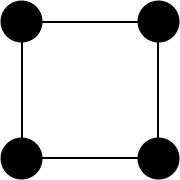
\includegraphics[width=2cm]{bcc100}\quad
  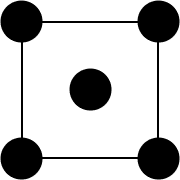
\includegraphics[width=2cm]{bcc110}\quad
  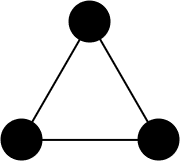
\includegraphics[width=2cm]{bcc111}
  \caption{BCC 100, 110, and 111 Planes}
  \label{fig:n}
\end{figure}
Note that the figure is not to scale, the 110 plane should be a bit wider than it is tall. In order to find the most dense we should consider defining a volume for each of the balls we see in the figure. The radius will be $\frac{1}{2}$ of the nearest neighbor distance in a bcc lattice, given in Kittel as:
\begin{align*}
  d_{bcc}=a\frac{\sqrt{3}}{2}
\end{align*}
So our radius will always be:
\begin{align*}
  r_{bcc}=a\frac{\sqrt{3}}{4}=\frac{d_{bcc}}{2}
\end{align*}
Let us also calculate the area of each of these planes, specifically their intersection with the unit cells. For (100) this is simple as the intersection is a face of the unit cell, so its area is:
\begin{align*}
  A_{100}=a^2
\end{align*}
As for (110) it is the same, except its width is the diagonal of a unit cell, so it has $a,a\sqrt{2}$ as its dimensions, giving:
\begin{align*}
  A_{110}=a^2\sqrt{2}
\end{align*}
Finally for (111) we can use the Pythagorean theorem to determine the side length is $a\sqrt{2}$, and it must be an equilateral triangle, so its area is:
\begin{align*}
  A_{111}=(a\sqrt{2})^2\frac{\sqrt{3}}{4}=a^2\frac{\sqrt{3}}{2}
\end{align*}
Now we simply need to count the number of lattice points in each intersection.

The 100 plane does not contain the center of the unit cell, so it only contains a quarter of a lattice point, so we get:
\begin{align*}
  n_{100}=\frac{1}{4}(4)=1
\end{align*}
The 110 plane contains the same amount as the 100 plane, but with the added body point. Thus we get:
\begin{align*}
  n_{110}=\frac{1}{4}(4)+1=2
\end{align*}
Finally for the 111 plane, using the symmetries of a triangle we can argue that each intersection has $\frac{1}{6}$ of a lattice point, but it does not contain the center point:
\begin{align*}
  n_{111}=\frac{1}{6}(3)=\frac{1}{2}
\end{align*}
Now for the density we need  the following:
\begin{align*}
  \rho=\frac{n\pi r_{bcc}^2}{A}
\end{align*}
So $\rho_{100}$ is:
\begin{align*}
  \rho_{100}&=\frac{1*\pi*a^2\frac{3}{16}}{a^2}\\
  &=\frac{3\pi}{16}
\end{align*}
And the other two:
\begin{align*}
  \rho_{110}&=\frac{2\pi a^2\frac{3}{16}}{a^2\sqrt{2}}\\
            &=\frac{3\pi}{16}\sqrt{2}\\
  \rho_{111}&=\frac{\frac{1}{2}\pi a^2\frac{3}{16}}{a^2\frac{\sqrt{3}}{2}}\\
            &=\frac{3\pi}{16}\frac{1}{\sqrt{3}}
\end{align*}
Clearly the densest is the 110 plane, as out of all of these numbers, $\sqrt{2}$ is the largest, ignoring the $\frac{3\pi}{16}$. 
\section*{Question 5}
If Ag has a single atom basis, then the number of conduction electrons is equal to the number of lattice points per unit cell. Using Kittel, the number of lattice points per cell in FCC is 4. So we have 4 conduction electrons per unit cell. The volume of the unit cell in a FCC structure is $a^3$, where $a$ is the lattice constant of $Ag$, given in various periodic tables as $4.0495$ \r{A} or $4.0495\times10^{-8}$ cm. Thus we can calculate $n$:
\begin{align*}
  n=\frac{4}{a^3}=\frac{4}{(4.0495\times10^{-8})}=
  \boxed{6.0236\times10^{22}\text{cm}^{-3}}
\end{align*}
\section*{Question 6}
This concept was used in problem 4, but for the planes. In Kittel table 2, the volume of the FCC conventional cell is given as $a^3$:
\begin{align*}
  V_{FCC}=a^3
\end{align*}
Next the number of lattice points per cell is known to be $4$, and the nearest neighbor distance is given as:
\begin{align*}
  d_{FCC}=\frac{a}{\sqrt{2}}
\end{align*}
The radius of one of the spheres will be half this distance:
\begin{align*}
  r_{FCC}=\frac{d_{FCC}}{2}=\frac{a}{2\sqrt{2}}
\end{align*}
So the volume of lattice points per unit cell is:
\begin{align*}
  V_{lp}=n\times\frac{4}{3}\pi r_{FCC}^3
\end{align*}
Where $n$ is lattice points per unit cell, plugging in our numbers:
\begin{align*}
  V_{lp}=a^3\frac{\pi}{3\sqrt{2}}
\end{align*}
So the packing fraction is this volume divided by the volume of the unit cell:
\begin{align*}
  \rho_{FCC}=\frac{V_{lp}}{V_{FCC}}=\boxed{\frac{\pi}{3\sqrt{2}}}
\end{align*}
Kittel gives it in a rationalized form:
\begin{align*}
  \rho_{FCC}=\frac{\pi}{3\sqrt{2}}\frac{\sqrt{2}}{\sqrt{2}}
  =\frac{\pi\sqrt{2}}{6}
\end{align*}
\end{document}